%-----------------------------------------------------------------------------------------------------------------------------------------------%
%	The MIT License (MIT)
%
%	Copyright (c) 2015 Jan Küster
%
%	Permission is hereby granted, free of charge, to any person obtaining a copy
%	of this software and associated documentation files (the "Software"), to deal
%	in the Software without restriction, including without limitation the rights
%	to use, copy, modify, merge, publish, distribute, sublicense, and/or sell
%	copies of the Software, and to permit persons to whom the Software is
%	furnished to do so, subject to the following conditions:
%	
%	THE SOFTWARE IS PROVIDED "AS IS", WITHOUT WARRANTY OF ANY KIND, EXPRESS OR
%	IMPLIED, INCLUDING BUT NOT LIMITED TO THE WARRANTIES OF MERCHANTABILITY,
%	FITNESS FOR A PARTICULAR PURPOSE AND NONINFRINGEMENT. IN NO EVENT SHALL THE
%	AUTHORS OR COPYRIGHT HOLDERS BE LIABLE FOR ANY CLAIM, DAMAGES OR OTHER
%	LIABILITY, WHETHER IN AN ACTION OF CONTRACT, TORT OR OTHERWISE, ARISING FROM,
%	OUT OF OR IN CONNECTION WITH THE SOFTWARE OR THE USE OR OTHER DEALINGS IN
%	THE SOFTWARE.
%	
%
%-----------------------------------------------------------------------------------------------------------------------------------------------%


%============================================================================%
%
%	DOCUMENT DEFINITION
%
%============================================================================%

%we use article class because we want to fully customize the page and dont use a cv template
\documentclass[10pt,A4]{article}	

\newcommand{\comment}[1]{}

%----------------------------------------------------------------------------------------
%	ENCODING
%----------------------------------------------------------------------------------------

%we use utf8 since we want to build from any machine
\usepackage[utf8]{inputenc}		

%----------------------------------------------------------------------------------------
%	LOGIC
%----------------------------------------------------------------------------------------

% provides \isempty test
\usepackage{xifthen}

% include hyperlinks
\usepackage{hyperref}

%----------------------------------------------------------------------------------------
%	FONT
%----------------------------------------------------------------------------------------

% some tex-live fonts - choose your own

%\usepackage[defaultsans]{droidsans}
%\usepackage[default]{comfortaa}
%\usepackage{cmbright}
\usepackage[default]{raleway}
%\usepackage{fetamont}
%\usepackage[default]{gillius}
%\usepackage[light,math]{iwona}
%\usepackage[thin]{roboto} 

% set font default
\renewcommand*\familydefault{\sfdefault} 	
\usepackage[T1]{fontenc}

% more font size definitions
\usepackage{moresize}		


%----------------------------------------------------------------------------------------
%	PAGE LAYOUT  DEFINITIONS
%----------------------------------------------------------------------------------------

%debug page outer frames
%\usepackage{showframe}			


%define page styles using geometry
\usepackage[a4paper]{geometry}		

% for example, change the margins to 2 inches all round
\geometry{top=.5cm, bottom=-.6cm, left=-0.1cm, right=0cm} 	

%use customized header
\usepackage{fancyhdr}				
\pagestyle{fancy}

%less space between header and content
\setlength{\headheight}{-5pt}		


%customize entries left, center and right
\lhead{}
\chead{}
\rhead{}

\newcommand{\padding}{1cm}
\newcommand{\innerwidth}{\linewidth-\padding-\padding}

%indentation is zero
\setlength{\parindent}{0mm}

%----------------------------------------------------------------------------------------
%	TABLE /ARRAY DEFINITIONS
%---------------------------------------------------------------------------------------- 

%for layouting tables
\usepackage{multicol}			
\usepackage{multirow}

%extended aligning of tabular cells
\usepackage{array}

\newcolumntype{x}[1]{%
>{\raggedleft\hspace{0pt}}p{#1}}%


%----------------------------------------------------------------------------------------
%	GRAPHICS DEFINITIONS
%---------------------------------------------------------------------------------------- 

%for header image
\usepackage{graphicx}

%for floating figures
\usepackage{wrapfig}
\usepackage{float}
%\floatstyle{boxed} 
%\restylefloat{figure}

%for drawing graphics		
\usepackage{tikz}				
\usetikzlibrary{shapes, backgrounds,mindmap, trees}


%----------------------------------------------------------------------------------------
%	Color DEFINITIONS
%---------------------------------------------------------------------------------------- 
\usepackage{transparent}
\usepackage{color}

%accent color
\definecolor{sectcol}{RGB}{255,150,0}

%dark background color
\definecolor{bgcol}{RGB}{110,110,110}

%light background / accent color
\definecolor{softcol}{RGB}{225,225,225}

% light bg
\definecolor{light}{RGB}{210, 210, 210}

%============================================================================%
%
%
%	DEFINITIONS
%
%
%============================================================================%

%----------------------------------------------------------------------------------------
% 	HEADER
%----------------------------------------------------------------------------------------

% remove top header line
\renewcommand{\headrulewidth}{0pt} 

%remove botttom header line
\renewcommand{\footrulewidth}{0pt}	  	

%remove pagenum
\renewcommand{\thepage}{}	

%remove section num		
\renewcommand{\thesection}{}			

%----------------------------------------------------------------------------------------
% 	ARROW GRAPHICS in Tikz
%----------------------------------------------------------------------------------------

% a six pointed arrow poiting to the left
\newcommand{\tzlarrow}{(0,0) -- (0.2,0) -- (0.3,0.2) -- (0.2,0.4) -- (0,0.4) -- (0.1,0.2) -- cycle;}	

% include the left arrow into a tikz picture
% param1: fill color
%
\newcommand{\larrow}[1]
{\begin{tikzpicture}[scale=0.58]
	 \filldraw[fill=#1!100,draw=#1!100!black]  \tzlarrow
 \end{tikzpicture}
}

% a six pointed arrow poiting to the right
\newcommand{\tzrarrow}{ (0,0.2) -- (0.1,0) -- (0.3,0) -- (0.2,0.2) -- (0.3,0.4) -- (0.1,0.4) -- cycle;}

% include the right arrow into a tikz picture
% param1: fill color
%
\newcommand{\rarrow}[1]
{\begin{tikzpicture}[scale=0.7]
	 \filldraw[fill=#1!100,draw=#1!100!black]  \tzrarrow
 \end{tikzpicture}
}



%----------------------------------------------------------------------------------------
%	custom sections
%----------------------------------------------------------------------------------------

% create a coloured box with arrow and title as cv section headline
% param 1: section title
%
\newcommand{\cvsection}[1]
{
\colorbox{sectcol}{\mystrut \makebox[1\linewidth][l]{
\larrow{bgcol} \hspace{-8pt} \larrow{bgcol} \hspace{-8pt} \larrow{bgcol} \textcolor{white}{\textbf{#1}}\hspace{4pt}
}}\\
}

%create a coloured arrow with title as cv meta section section
% param 1: meta section title
%
\newcommand{\metasection}[2]
{
\begin{tabular*}{1\textwidth}{p{2cm} p{11cm}}
\larrow{bgcol}	\normalsize{\textcolor{sectcol}{#1}}&#2\\[8pt]
\end{tabular*}
}

%----------------------------------------------------------------------------------------
%	 CV EVENT
%----------------------------------------------------------------------------------------

% creates a stretched box as cv entry headline followed by two paragraphs about 
% the work you did
% param 1:	event time i.e. 2014 or 2011-2014 etc.
% param 2:	event name (what did you do?)
% param 3:	institution (where did you work / study)
% param 4:	what was your position
% param 5:	some words about your contributions
%
\newcommand{\cvevent}[5]
{
\vspace{8pt}
	\begin{tabular*}{0.6\linewidth}{ p{12cm} x{3cm}}
\textbf{#2} \textcolor{bgcol}{(#3)}&\textcolor{bgcol}{#1}\\[4pt]
	\end{tabular*}
\vspace{-12pt}
\textcolor{softcol}{\hrule}
\vspace{6pt}
	\begin{tabular*}{1\textwidth}{l}
		 \larrow{sectcol}  #4\\[4.5pt]
		 \larrow{sectcol}  #5\\[6pt]
	\end{tabular*}
\vspace{-4pt}
}

% creates a stretched box as 
\newcommand{\cveventmeta}[2]
{
	\mbox{\mystrut \hspace{87pt}\textit{#1}}\\
	#2
}

%----------------------------------------------------------------------------------------
% CUSTOM STRUT FOR EMPTY BOXES
%----------------------------------------- -----------------------------------------------
\newcommand{\mystrut}{\rule[-.3\baselineskip]{0pt}{\baselineskip}}

%----------------------------------------------------------------------------------------
% CUSTOM LOREM IPSUM
%----------------------------------------------------------------------------------------
\newcommand{\lorem}
{Lorem ipsum dolor sit amet, consectetur adipiscing elit. Donec a diam lectus.}



%============================================================================%
%
%
%
%	DOCUMENT CONTENT
%
%
%
%============================================================================%
\begin{document}

%use our custom fancy header definitions
\pagestyle{fancy}	

%----------------------------------------------------------------------------------------
% HEADLINE / BASIC INFORMATION
%----------------------------------------------------------------------------------------
\fcolorbox{bgcol}{bgcol}{
\begin{minipage}[c][0.085\textheight][t]{\linewidth}
\begin{center}
	\vspace{14pt}
	\textcolor{light}{\small{Software Engineer and Part Qualified Actuary $\cdot$  Cork, Ireland  $\cdot$  \href{mailto:barry7ie.jobs@gmail.com}{barry7ie.jobs@gmail.com}  $\cdot$ +353 (0) 87 255 3482}}\\
	\HUGE{\textcolor{white}{\textsc{Barry O' Farrell}} } \textcolor{sectcol}{\rule[-1mm]{1mm}{0.9cm}} \HUGE{\textcolor{white}{\textsc{Curriculum Vitae}} }
\end{center}
\end{minipage}}\\[-4pt]
%----------------------------------------------------------------------------------------
% SUMMARY
%----------------------------------------------------------------------------------------
\fcolorbox{sectcol}{sectcol}{
\begin{minipage}[c][0.03\textheight][t]{\linewidth}
\vspace{-3pt}
\begin{center}
\parbox[b]{0.75\linewidth}{
	\begin{center}
	\large
	\larrow{bgcol}\larrow{bgcol} \textcolor{white}{I am open to full-time positions across all industries and sectors.} \rarrow{bgcol}\rarrow{bgcol}
	\end{center}
}
\end{center}
\end{minipage}}\\[-4pt]
%----------------------------------------------------------------------------------------
% META
%----------------------------------------------------------------------------------------
\fcolorbox{white}{white}{
\begin{minipage}[c][0.16\textheight][t]{\linewidth}
\vspace{8pt}
\begin{center}
\parbox[c]{\innerwidth}{
	%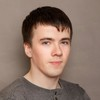
\includegraphics[trim= 320 130 460 210,clip,width=0.2\linewidth]{0.jpg}
	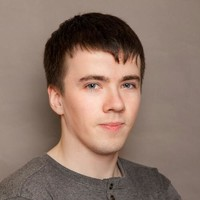
\includegraphics[width=0.2\linewidth]{1.jpg}
	\hspace{8pt}
	\parbox[b]{5cm}{
	\metasection{Status:}{MSc. Info Sec. Student, HDip. Applied Computing, BSc. Financial Mathematics \& Actuarial Science}
	\metasection{Fields:}{Data Analysis, Software Development, Cyber Security, Accessibility} 
	\metasection{Lang.:}{Python, Bash, HTML5, CSS3, Javascript, LAMP, Postgresql, Selenium}
	\metasection{Tools:}{Git, Sourcetree,  Terminal, DPI 15 + NatLink + Dragonfly + Caster, MS Office, MS SQL Server 2008, SSIS}
	\metasection{Activities:}{Web Scraping, Coding by voice, information security}
	}
}
\end{center}
\end{minipage}}\\[-4pt]
%----------------------------------------------------------------------------------------
% EXPERIENCE
%----------------------------------------------------------------------------------------
\fcolorbox{light}{light}{
\begin{minipage}[c][0.67\textheight][t]{\linewidth}
\vspace{4pt}
\hspace{26pt}
\parbox[c]{0.75\linewidth}{
%
\cvevent{7/2016 - 9/2016}{Actuarial Analyst - ORSA Development}{MetLife, Dublin}{Development/refinement of existing SII models to hasten the ORSA production process }{Documentation of developing process}

%\textcolor{softcol}{\hrule}

%
\cvevent{4/2015 - 7/2016}{Actuarial Analyst - ORSA Production}{MetLife, Dublin}{Production of ORSA/FLAOR Projections. Automating and documenting these processes.}{Assisting in the training and guidance of more junior members of the team.}


%\textcolor{softcol}{\hrule}

%
\cvevent{8/2014 - 4/2015}{Actuarial Analyst - EMEA Projections}{MetLife, Dublin}{Consolidating existing Projection Models across the EMEA region}{Implementng agreed New Business Methodologies}

%\textcolor{softcol}{\hrule}

%
\cvevent{1/2013 - 7/2014}{Actuarial Analyst - Finanial Reporting}{MetLife, Dublin}{Reporting quarterly reserves}{Analysing reasons for changes in reserves between quarters}

%\textcolor{softcol}{\hrule}

%
\cvevent{2008 - 2012}{Accounts Assistant}{Doreen's Bakery, Cork}{Inputted sales data in Excel \& via Electronic Data Interchange }{Met monthly deadlines to have invoices correct \& ready for dispatch}

%
\cvevent{6/2011 - 8/2011}{Reward Advisory Services - Summer Intern}{PwC, Dublin}{Compiled ‘Executive Remuneration’ database}{Involved in analysis of client remuneration data}

\cvevent{7/2010 - 9/2010}{Actuarial Summer Intern}{Irish Life Group, Dublin}{Re-evaluated several hundred pension policies, before a very strict deadline }{Reassessed calculations, after management changes, to the agreed valuation policy}

	


}
\hspace{18pt}
\textcolor{sectcol}{\rule[-3.2cm]{2pt}{7cm}}
\hspace{12pt}
\rotatebox[origin=c]{270}{\HUGE \textsc{Experience}}
\end{minipage}}\\[-4pt]
%----------------------------------------------------------------------------------------
% SUMMARY
%----------------------------------------------------------------------------------------
%\comment{
\fcolorbox{bgcol}{bgcol}{
\begin{minipage}[c][0.03\textheight][t]{\linewidth}
\vspace{-3pt}
\begin{center}
\parbox[b]{0.75\linewidth}{
	\begin{center}
	\large
	\textcolor{white}{Check out my LinkedIn profile at - } \textcolor{sectcol}{\textbf{\href{https://linkedin.com/in/barry-o-farrell}{linkedin.com/in/barry-o-farrell}}}
	\end{center}
}
\end{center}
\end{minipage}}\\[-4pt]
%}

%----------------------------------------------------------------------------------------
% HEADLINE / BASIC INFORMATION
%----------------------------------------------------------------------------------------
\fcolorbox{bgcol}{bgcol}{
	\begin{minipage}[c][0.085\textheight][t]{\linewidth}
		\begin{center}
			\vspace{14pt}
			\textcolor{light}{\small{Software Engineer and Part Qualified Actuary $\cdot$  Cork, Ireland  $\cdot$  \href{mailto:barry7ie.jobs@gmail.com}{barry7ie.jobs@gmail.com}  $\cdot$ +353 (0) 87 255 3482}}\\
			\HUGE{\textcolor{white}{\textsc{Barry O' Farrell}} } \textcolor{sectcol}{\rule[-1mm]{1mm}{0.9cm}} \HUGE{\textcolor{white}{\textsc{Curriculum Vitae}} }
		\end{center}
\end{minipage}}\\[-4pt]
%----------------------------------------------------------------------------------------
% SUMMARY
%----------------------------------------------------------------------------------------
\fcolorbox{sectcol}{sectcol}{
	\begin{minipage}[c][0.03\textheight][t]{\linewidth}
		\vspace{-3pt}
		\begin{center}
			\parbox[b]{0.75\linewidth}{
				\begin{center}
					\large
					\larrow{bgcol}\larrow{bgcol} \textcolor{white}{I am open to full-time positions across all industries and sectors.} \rarrow{bgcol}\rarrow{bgcol}
				\end{center}
			}
		\end{center}
\end{minipage}}\\[-4pt]
%----------------------------------------------------------------------------------------
% META
%----------------------------------------------------------------------------------------
\fcolorbox{white}{white}{
	\begin{minipage}[c][0.16\textheight][t]{\linewidth}
		\vspace{8pt}
		\begin{center}
			\parbox[c]{\innerwidth}{
				%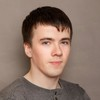
\includegraphics[trim= 320 130 460 210,clip,width=0.2\linewidth]{0.jpg}
				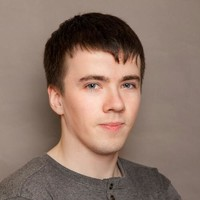
\includegraphics[width=0.2\linewidth]{1.jpg}
				\hspace{8pt}
				\parbox[b]{5cm}{
					\metasection{Status:}{MSc. Info Sec. Student, HDip. Applied Computing, BSc. Financial Mathematics \& Actuarial Science}
					\metasection{Fields:}{Data Analysis, Software Development, Cyber Security, Accessibility} 
					\metasection{Lang.:}{Python, Bash, HTML5, CSS3, Javascript, LAMP, Postgresql, Selenium}
					\metasection{Tools:}{Git, Sourcetree,  Terminal, DPI 15 + NatLink + Dragonfly + Caster, MS Office, MS SQL Server 2008, SSIS}
					\metasection{Activities:}{Web Scraping, Coding by voice, information security}
				}
			}
		\end{center}
\end{minipage}}\\[-4pt]
%----------------------------------------------------------------------------------------A


%----------------------------------------------------------------------------------------
% EDUCATION
%----------------------------------------------------------------------------------------
\fcolorbox{white}{white}{
\begin{minipage}[c][0.675\textheight][t]{\linewidth}
\vspace{1pt}
\hspace{26pt}
\parbox[c]{0.75\linewidth}{
%\cvsection{Education}

\cvevent{2018 - Present}{Student MSc. Info Security}{Cork Institute Of Technology}{Malware analysis, Offensive security, Scripting}{Network and digital forensics, cryptography, Security management and law}

%\textcolor{softcol}{\hrule}

%
\cvevent{2016 - 2017}{Higher Diploma Applied Computing}{University College Cork}{Python, HTML5, CSS3, RWD, Javascript, Server-side programming with Python}{Photoplus, XVI32 Hex editor images, Logic circuits \& basic Assembly language, PHP, MySQL}

%\textcolor{softcol}{\hrule}

%
\cvevent{2012 - 1/2013}{Incomplete MSc. Mathematical modelling \& scientific computing}{UCC}{Incomplete, due to taking job offer from MetLife in January 2013}{First semester subjects covered: Mathematica, Cellular Automata, OOP (using C Sharp )}

%
\cvevent{2008 - 2012}{BSc. Financial Maths \& Actuarial Science}{University College Cork}{Financial mathematics, actuarial science, Statistics}{Mathematics, Applied mathematics}

%\textcolor{softcol}{\hrule}

%
\cvevent{2002 - 2008}{Secondary school}{Coláiste an Spoioraid Naoimh, Cork}{(2008) Leaving certificate - 600 points (6A1s, 2A2s)}{Subjects: English, Irish, French, maths, physics, chemistry, technical drawing, applied maths}
}
\hspace{18pt}
\textcolor{sectcol}{\rule[-3.2cm]{2pt}{7cm}}
\hspace{12pt}
\rotatebox[origin=c]{270}{\HUGE \textsc{Education}}
\end{minipage}}\\[-4pt]
%---------------------------------------------------------------------------------------
%	QR CODE (optional)
%----------------------------------------------------------------------------------------
%\vspace{-136pt}
%\hspace{0.75\linewidth}
%\includegraphics[width=103pt]{qrcode}
%\normalsize
%\vspace{88pt}



%-------------------------------------------------------------------------------------------------
% FOOTER
%--------------------------------------------------------------------------------------------------
\fcolorbox{bgcol}{bgcol}{
\begin{minipage}[c][0.01\textheight][t]{\linewidth}
\vspace{-8pt}
\begin{center}
\parbox[b]{0.75\linewidth}{
	\begin{center}
	 \textcolor{white}{For more details - LinkedIn profile  } \textcolor{white}{$\cdot$} \textcolor{white}{\href{https://linkedin.com/in/barry-o-farrell}{linkedin.com/in/barry-o-farrell}}
	\end{center}
}
\end{center}
\end{minipage}}
%============================================================================%
%
%
%
%	DOCUMENT END
%
%
%
%============================================================================%
\end{document}
